\subsection{Communication} \label{subsec:Communication}
The Main Processor and Sample Control modules need a communication interface in order to set control settings for the ADCs, DAC in the FPGA's internal registers and to retrieve stored ADC samples.The ADCs and DAC \todo{Vi mangler at redegøre for det her valg.} both have 16 bits of resolution and a 16 bit wide parallel bus between the FPGA and MCU will be used to transfer the data as shown on figure \refq{fig_7_2_1_CommBus}.

\begin{figure}[H]
    \centering
    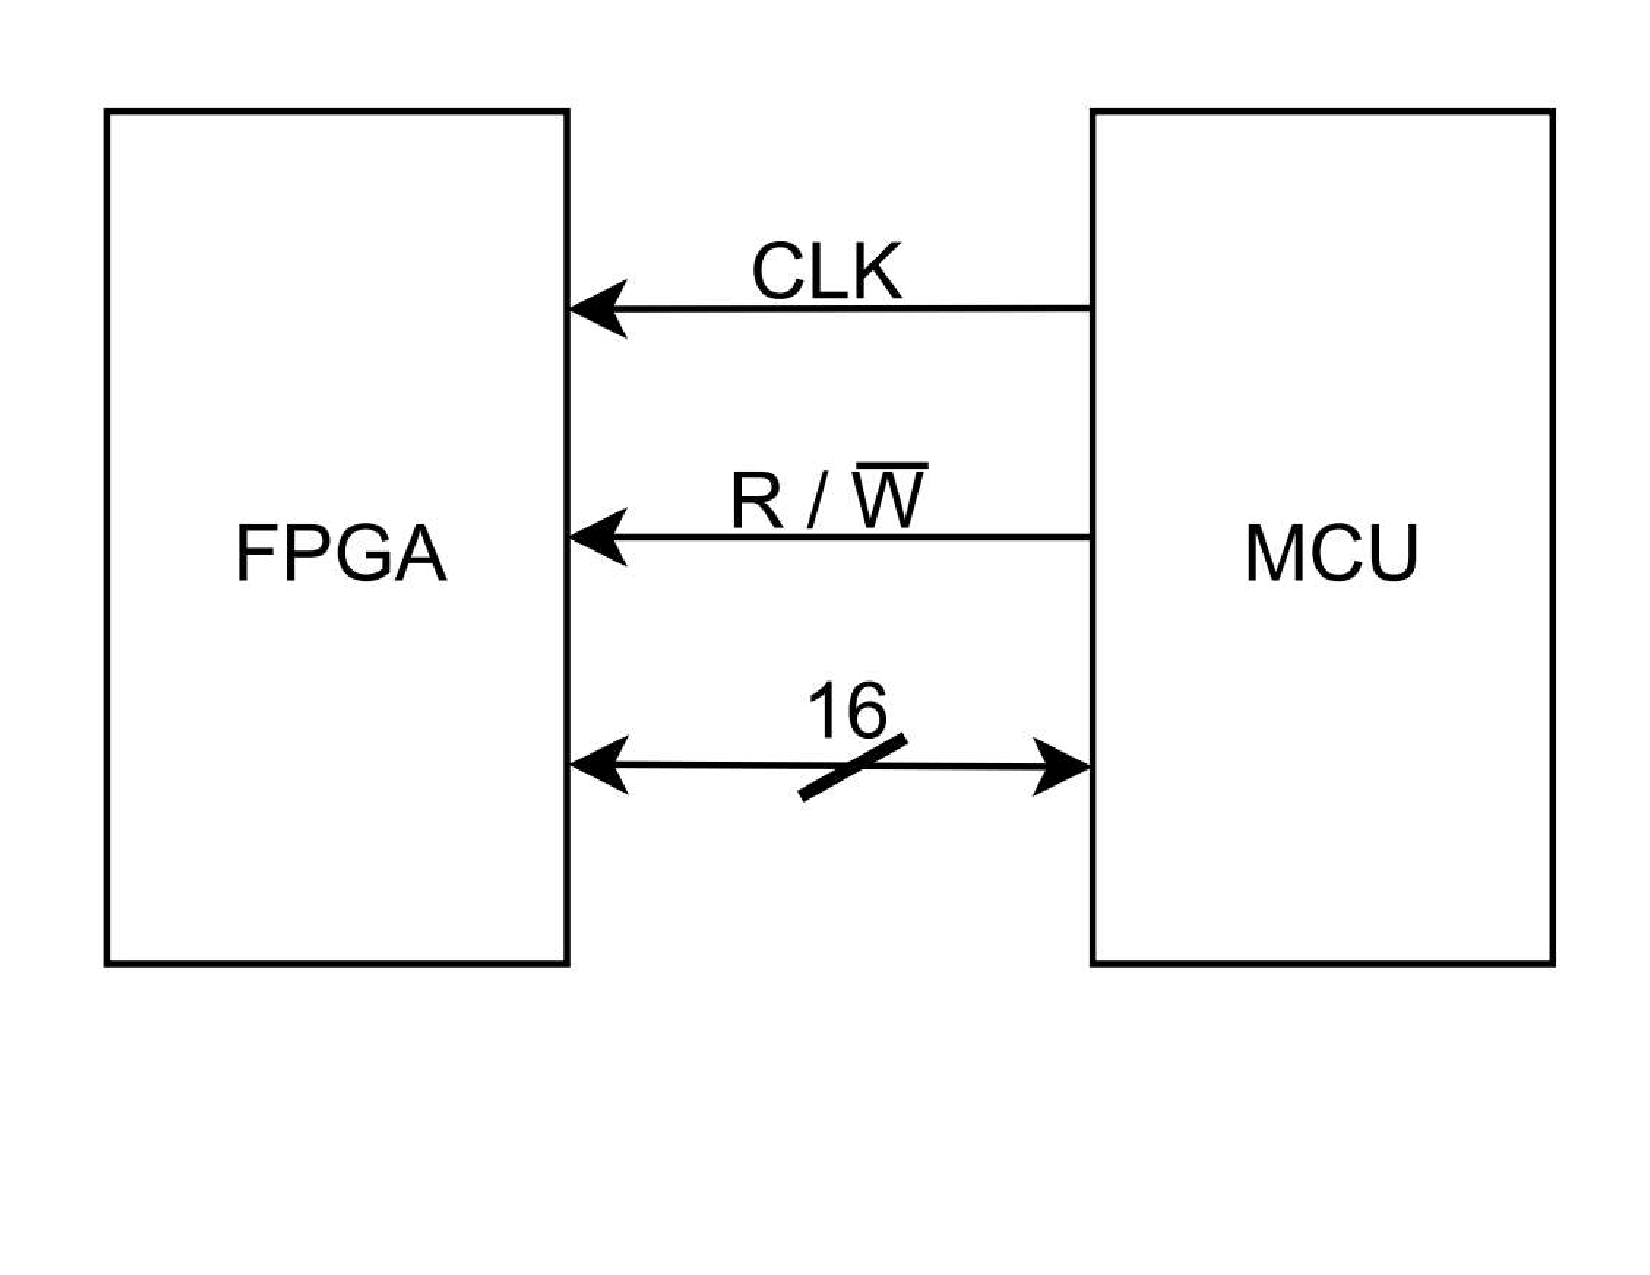
\includegraphics[clip, trim=0 100 0 0, width=0.5\textwidth]{Sections/7_SystemDesign/Figures/7_2_1_CommunicationBus.pdf}
    \caption{The communication bus connection the FPGA and microcontroller. It uses a 16 bit databus, a long with a CLK and a read/write control signal.}
    \label{fig_7_2_1_CommBus}
\end{figure}

The microcontroller is always going to be the master that has to initiate communication and the FPGA is always the slave. The microcontroller is controlling the read/write and CLK control signals necessary for the communication to work. The Read-write pin is, when  RW = '0', in write mode and in read mode when RW = '1'. Data is clocked in and out on the rising edges of the CLK. 

If the MCU wants to write some value into a register it must first CLK in an address into the FPGA before it can CLK in any data, as shown on figure \refq{fig_7_2_1_CommWrite}. 
\begin{figure}[H]
    \centering
    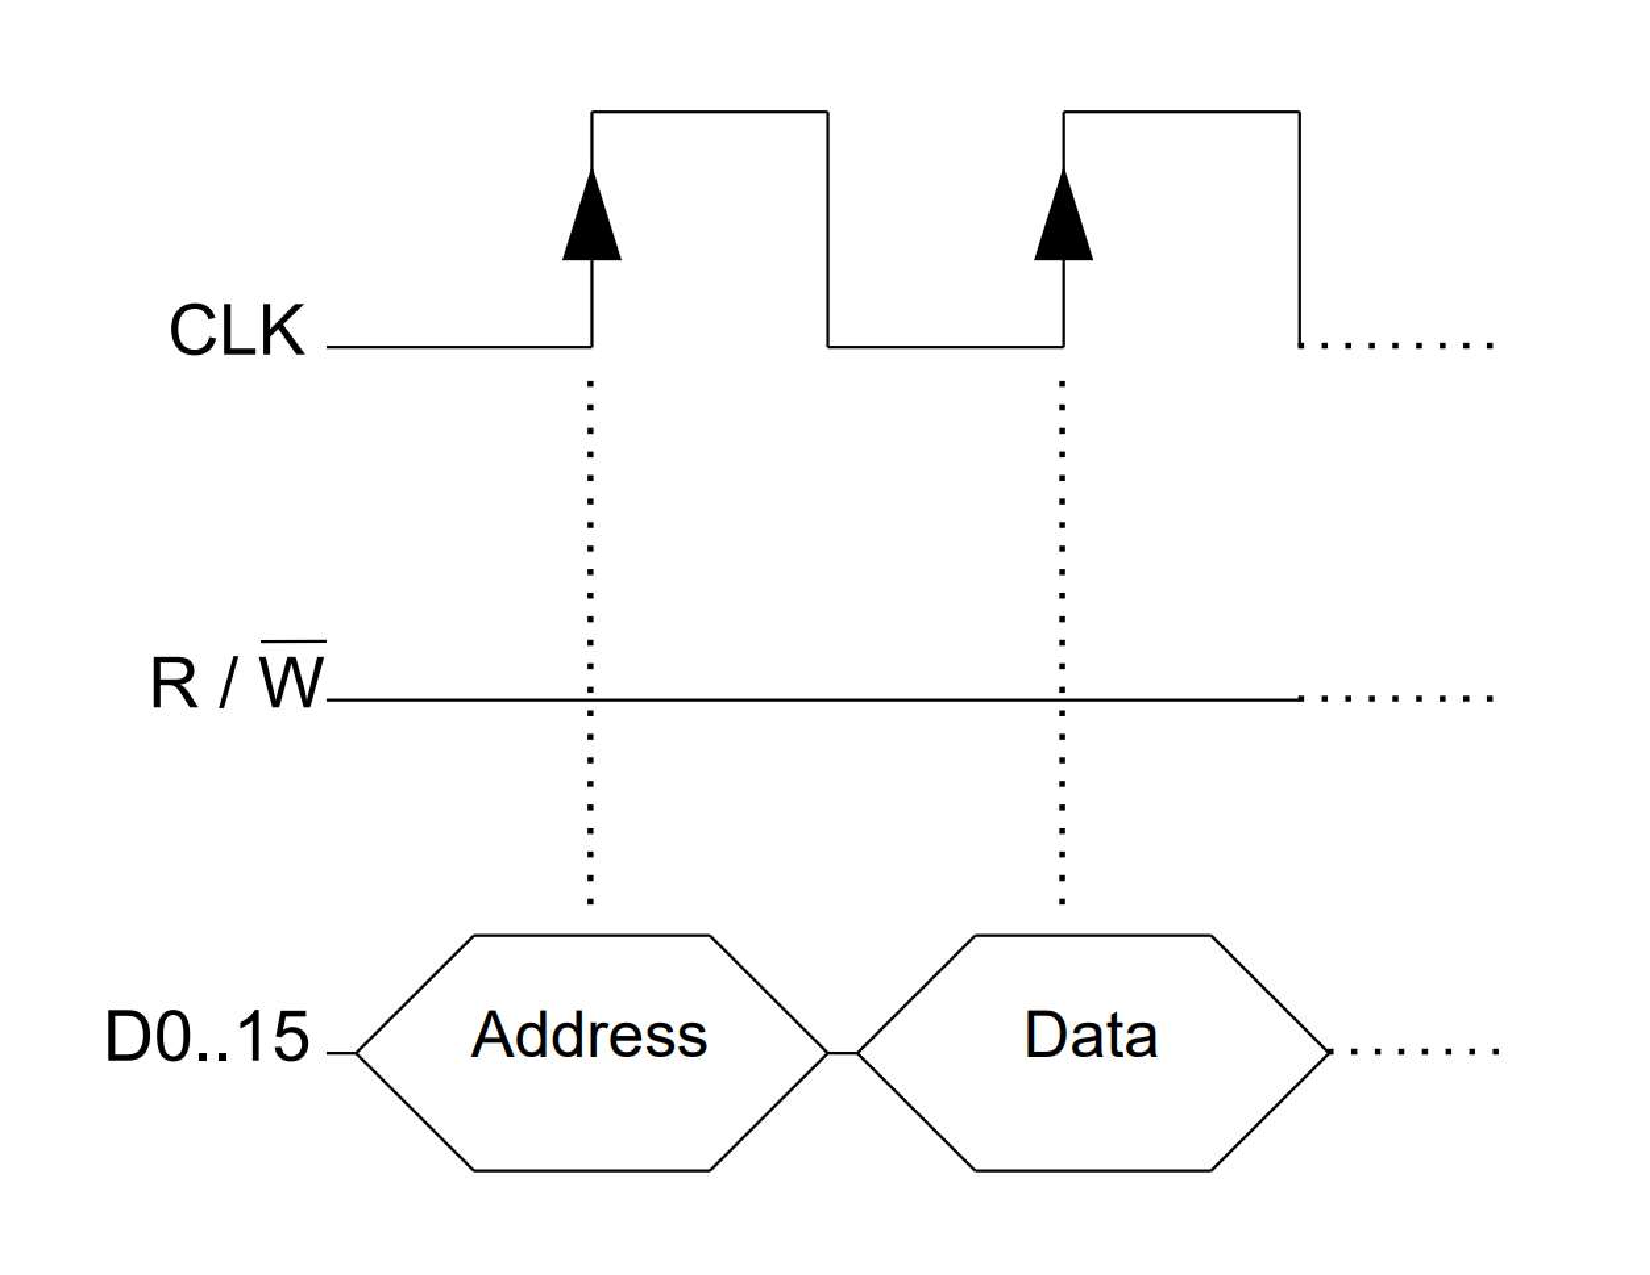
\includegraphics[clip, trim=0 50 0 0, width=0.5\textwidth]{Sections/7_SystemDesign/Figures/7_2_1_CommWrite.pdf}
    \caption{In order to write to the FPGA, the MCU must first set RW ='0' then set the 16 bit bus to the desired address and generate a single CLK pulse. The address is clocked into the FPGA on a rising edge. To write data into the address; the MCU sets 16 bit data on the bus and then generate a single clock pulse. Data is clocked into the FPGA on a rising edge.}
    \label{fig_7_2_1_CommWrite}
\end{figure}

Note how on figure \refq{fig_7_2_1_CommWrite} D0..D15 should have settled before the MCU tries to clock in any value. This will be ensured by design as the signals for the communication are generated sequentially in software on the MCU. They are not hardware controlled and there will be a minimum of \SIQ{35.8}{\nano\second} between D0..D15 and CLK as shown in appendix \refq{App:MicrocontrollerConsiderations} and significantly more if the MCU wants to read from the FPGA.

If the MCU wants to read from the FPGA it must first CLK in an address in the same way as for a write operation, then change it's D0..D15 output pins to input pins and set RW '1'. The following CLK will cause the FPGA to set the data unto the bus pins as shown on figure xyz

\begin{figure}[H]
    \centering
    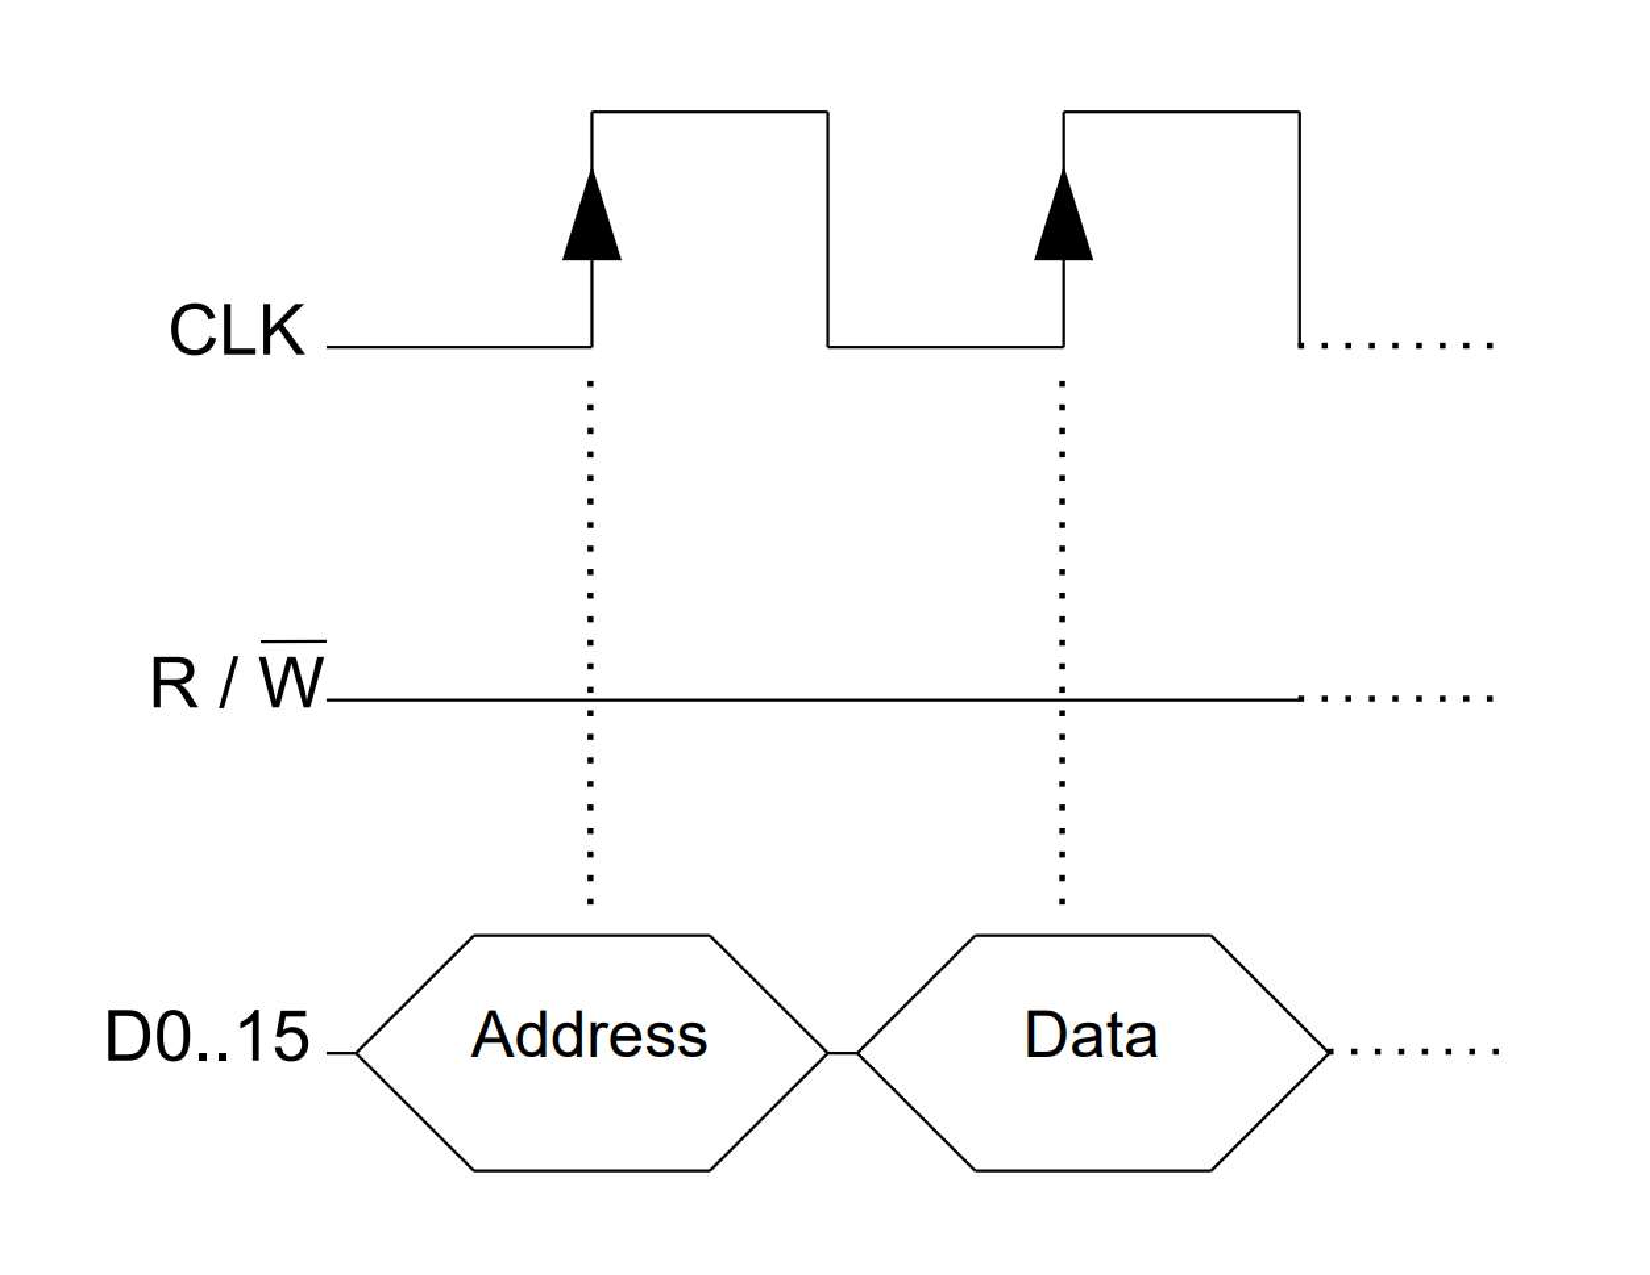
\includegraphics[clip, trim=0 50 0 0, width=0.5\textwidth]{Sections/7_SystemDesign/Figures/7_2_1_CommWrite.pdf}
    \caption{In order to write to the FPGA, the MCU must first set RW ='0' then set the 16 bit bus to the desired address and generate a single CLK pulse. The address is clocked into the FPGA on a rising edge. To write data into the address; the MCU sets 16 bit data on the bus and then generate a single clock pulse. Data is clocked into the FPGA on a rising edge.}
    \label{fig_7_2_1_CommWrite}
\end{figure}
